\begin{figure*}[t]

\centering

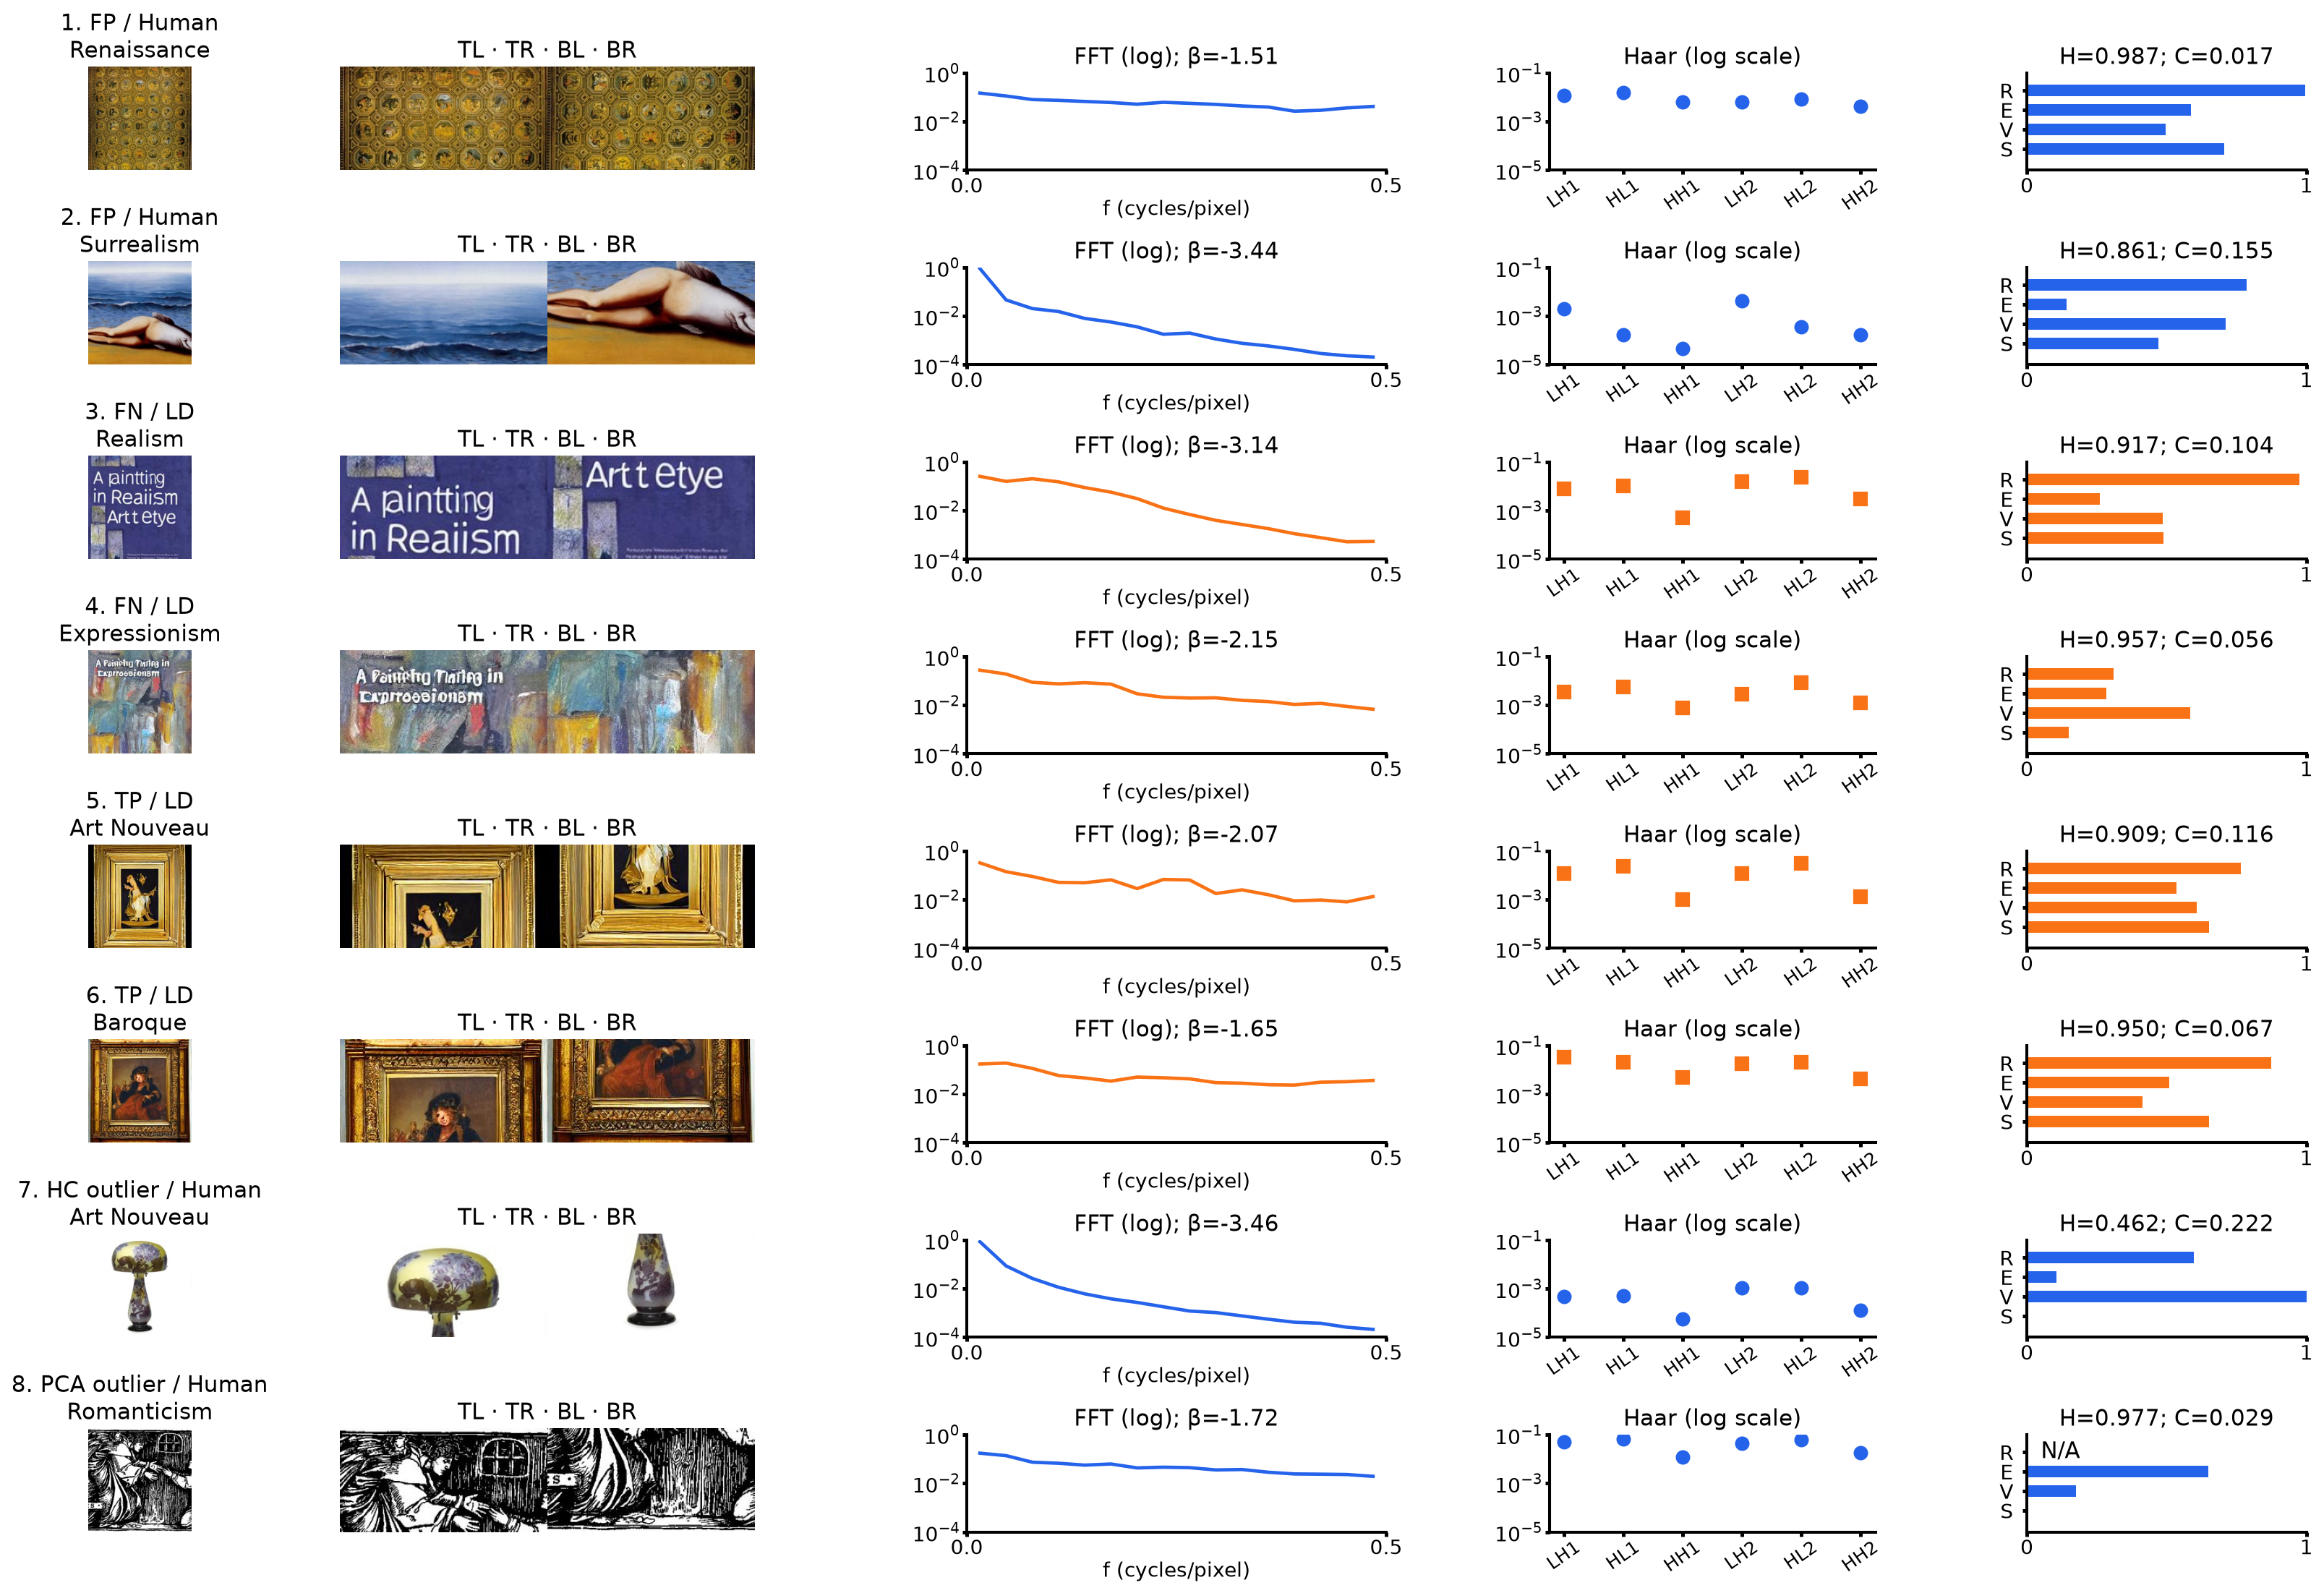
\includegraphics[width=\textwidth,height=4.9in,keepaspectratio]{figure_12.png}

\caption{Eight purposive cases, not prevalence estimates; FP/FN/TP refer to release labels. FFT rows share 10$^{-4}$--1 and Haar rows 10$^{-5}$--10$^{-1}$, both logarithmic. S = saturation, V = value, E = edge density, R = hue concentration (N/A when undefined).}\label{fig:f12}

\end{figure*}